\documentclass[tikz,border=4mm]{standalone}
      \usepackage{tikz}
      \usetikzlibrary{arrows.meta,positioning,calc,shapes.geometric}
      \begin{document}
      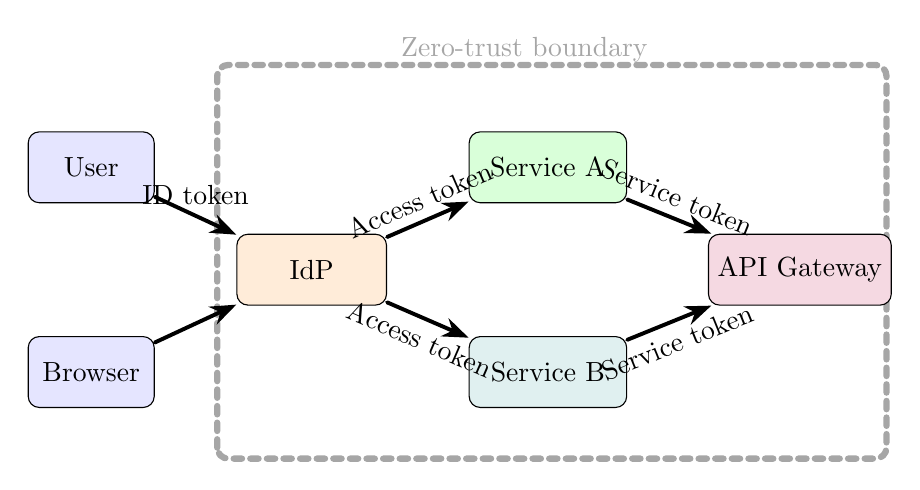
\begin{tikzpicture}[>=Stealth, line cap=round, line join=round]

\draw[rounded corners, dashed, gray!70, line width=0.08cm] (3.0,2.2) rectangle (11.5,7.2);
\node[draw, rounded corners, fill=blue!10, minimum width=1.6cm, minimum height=0.9cm] (user) at (1.4,5.9) {User};
\node[draw, rounded corners, fill=blue!10, minimum width=1.6cm, minimum height=0.9cm] (browser) at (1.4,3.3) {Browser};
\node[draw, rounded corners, fill=orange!15, minimum width=1.9cm, minimum height=0.9cm] (idp) at (4.2,4.6) {IdP};
\node[draw, rounded corners, fill=green!15, minimum width=2.0cm, minimum height=0.9cm] (svcA) at (7.2,5.9) {Service A};
\node[draw, rounded corners, fill=teal!12, minimum width=2.0cm, minimum height=0.9cm] (svcB) at (7.2,3.3) {Service B};
\node[draw, rounded corners, fill=purple!15, minimum width=2.1cm, minimum height=0.9cm] (gw) at (10.4,4.6) {API Gateway};
\node[gray!70] at (6.9,7.4) {Zero-trust boundary};
\draw[->, line width=0.05cm] (user) -- node[above] {ID token} (idp);
\draw[->, line width=0.05cm] (browser) -- (idp);
\draw[->, line width=0.05cm] (idp) -- node[above, sloped] {Access token} (svcA);
\draw[->, line width=0.05cm] (idp) -- node[below, sloped] {Access token} (svcB);
\draw[->, line width=0.05cm] (svcA) -- node[above, sloped] {Service token} (gw);
\draw[->, line width=0.05cm] (svcB) -- node[below, sloped] {Service token} (gw);

      \end{tikzpicture}
      \end{document}
